\documentclass[11pt,article]{article}
\usepackage[utf8]{inputenc}
\usepackage[T1]{fontenc} % caractères accentués en entrée, dans emacs
\usepackage[french]{babel}
\FrenchFootnotes
\selectlanguage{french}
\usepackage{a4wide} % possibilité d'utiliser toute la page a4
% selon GUT#33, avril 2007, page 13, empagement
% largeur des textes (ou justification) = 15cm
% hauteur du rectangle d'empagement = 23cm
% blanc de couture = 2/5 (21-15) = 2.4 = inner = right
% blanc de grand fond = 3/5 (21-15) = outer = left
% blanc de tête = 2/5 (29,7-23) = top
% blanc de pied = 3/5 (29,7-23) = bottom
%\usepackage[a4paper,twoside=true,right=2.4cm,left=3.6cm,top=2.68cm,bottom=4.02cm]{geometry} 
% selon CFSE 2006
% - largeur des textes (ou justification) : 16cm (2cm de marge, et 1cm
%   de reliure) ;
% - hauteur des textes, y compris les notes : 23cm (2,5cm de marge
%   haute et 2cm de marge basse) ; 1ère page de : 36pts
%   d'espacement avant le titre ;
\oddsidemargin   -4mm           % 3cm a gauche des impaires
\evensidemargin   4mm           % 2cm a gauche des paires
\topmargin       -18mm          % 2.5cm en haut
\headheight       13mm          % taille de l'entete (lignes)
\headsep          24pt          % espace entre entete et texte
\footskip         30pt          % espace entre pied de page et texte
\textheight      230mm          % longeur du texte
\textwidth       160mm          % largeur du texte
\parskip 1pt                    % pas de sauts entre paragraphes
%\parindent 0pt                  % largeur de l'indentation
\usepackage{graphicx} % figure postcript avec latex,
		      % figure png avec pdflatex, au lieu d'utiliser epsfig
\usepackage[usenames,dvipsnames,table]{xcolor}
\usepackage{paralist}
\usepackage{ifthen}
\usepackage{amssymb}
\usepackage{amsfonts}
\usepackage{amsmath}
\usepackage{eurosym}
\usepackage{textcomp}
\usepackage{listings}
\lstset{language=Java,numbers=left,numberstyle=\tiny,stepnumber=4,numbersep=5pt,xleftmargin=5pt}

\usepackage{alltt}
\usepackage{longtable}

% adjust word spacing less strictly
% as result, some spaces between words may be a bit too large,
% but long words will be placed properly.
\sloppy

\newcommand{\cmt}[1]{\texttt{<}\textbf{--~#1~--}\texttt{>}}

\usepackage{lineno}
\usepackage{xspace}

\setlength{\marginparwidth}{1cm}
\setlength{\marginparsep}{10pt}
\reversemarginpar
\newcounter{usecasehaute}
\newcommand{\haute}{Haute}
\newcommand{\moyenne}{Moyenne}
\newcommand{\basse}{basse}
\newcommand{\usecase}[4]{\item \marginpar{\vspace{5pt}\ifthenelse{\equal{#1}{Haute}}{\centering\textsc{#1}\stepcounter{usecasehaute}\newline n$^{\circ}$ \theusecasehaute}{\ifthenelse{\equal{#1}{Moyenne}}{#1}{\small #1}}} #2 \begin{itemize}\item précondition~: #3 \item postcondition~: #4\end{itemize}}
\newcommand{\priorityusecase}[2]{\item \marginpar{\vspace{5pt}\ifthenelse{\equal{#1}{Haute}}{\centering\textsc{#1}\stepcounter{usecasehaute}\newline n$^{\circ}$ \theusecasehaute}{\ifthenelse{\equal{#1}{Moyenne}}{#1}{\small #1}}} #2}
\newcommand{\casusecase}[4]{\usecase{#1}{#2}{#3}{#4}}

\newcommand{\nullvalue}{\textsf{null}\xspace}
\newcommand{\emptyvalue}{\ensuremath\mathrm{vide}}
\newcommand{\invariant}{\ensuremath\mathrm{invariant}}

\begin{document}
\title{Projet CSC4102: <<~Suivi d'activité de projet~>>}
\author{Nom Prénom Étudiant1 et Nom Prénom Étudiants2}
\date{Année 2022--2023~---~\today}
\maketitle

\vfill

\tableofcontents

\newpage

\section{Spécification}

\subsection{Diagrammes de cas d'utilisation}

{\noindent\color{red}\textbf{Le diagramme suivant est à compléter. Ce
    commentaire est à retirer ensuite.}}

{\noindent\color{red}\textbf{Comme il y aura de nombreux cas
    d'utilisation, nous demandons que vous fassiez plusieurs
    diagrammes de cas d'utilisation afin d'avoir des diagrammes
    lisibles au format A4/portrait.}}

\begin{figure}[!ht]
\begin{center}
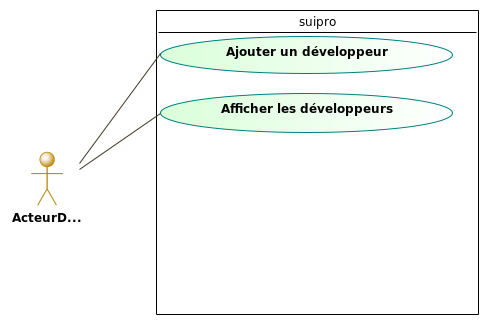
\includegraphics[scale=0.6]{Diagrammes/suipro_uml_diag_cas_utilisation_partie_developpeur}
\caption{Diagramme de cas d'utilisation~---~partie développeur.}
\end{center}
\label{usecase_modelio}
\end{figure}

\newpage

\subsection{Priorités, et préconditions et postconditions des cas d'utilisation}

%% Les priorités des cas d'utilisation pour le sprint~1 sont choisies
%% avec les règles de bon sens suivantes:
%% \begin{compactitem}
%% \item pour retirer une entité du système, elle doit y être. La
%% priorité de l'ajout est donc supérieure ou égale à la priorité du
%% retrait;
%% \item pour lister les entités d'un type donné, elles doivent y être. La
%% priorité de l'ajout est donc supérieure ou égale à la priorité du
%% listage;
%% \item il est \textit{a priori} possible, c.-à-d. sans raison
%% contraire, de démontrer la mise en œuvre d'un sous-ensemble des
%% fonctionnalités du système, et plus particulièrement la prise en
%% compte des principales règles de gestion, sans les retraits ou les
%% listages.
%% \item la possibilité de lister aide au déverminage de l'application
%% pendant les activités d'exécution des tests de validation.
%% \end{compactitem}
%% Par conséquent, les cas d'utilisation d'ajout sont \textit{a priori}
%% de priorité <<~haute~>>, ceux de listage de priorité <<~moyenne~>>, et
%% ceux de retrait de priorité <<~basse~>>.

%% \bigskip

%% Dans la suite, nous donnons les préconditions et postconditions pour
%% les cas d'utilisation de priorité <<~\haute~>>. Pour les autres, nous
%% indiquons uniquement leur niveau de priorité.

%% \bigskip

{\noindent\color{red}\textbf{La liste de préconditions et
    postconditions suivante est à modifier et compléter. Ce
    commentaire est à retirer ensuite.}}

\bigskip

\bigskip

Voici les préconditions et postconditions des cas d'utilisation du
premier sprint:
\begin{compactitem}
\usecase{\haute}{Ajouter un développeur}
        %% précondition
        {\newline
          $\land$ alias du développeur bien formé (non \nullvalue
          et non vide)
          \newline
          $\land$ nom bien formé (non \nullvalue et non vide)
          \newline
          $\land$ prénom bien formé (non \nullvalue et non vide)
          \newline
          $\land$ développeur avec cet alias inexistant}
        %% postcondition
        {développeur avec cet alias existant}

\smallskip

\priorityusecase{\moyenne}{Lister les développeurs}
 
\end{compactitem}

\newpage

\section{Préparation des tests de validation}

\subsection{Tables de décision des tests de validation}

La fiche programme du module CSC4102 ne permettant pas de développer
des tests de validation couvrant l'ensemble des cas d'utilisation de
l'application, les cas d'utilisation choisis sont de
priorité \textsc{Haute}.

\bigskip

{\noindent\color{red}\textbf{La section est à compléter avec les
    tables de décision d'autres cas d'utilisation. Ce commentaire est
    à retirer ensuite.}}

\begin{table}[htbp!]
\begin{tabular}{|p{0.6\linewidth}|c|c|c|c|c|}
\hline
Numéro de test
&1&2&3&4&5\\
\hline
\hline
Alias du développeur bien formé (non \nullvalue et non vide)
&F&T&T&T&T\\
\hline
Nom bien formé (non \nullvalue et non vide)
& &F&T&T&T\\
\hline
Prénom bien formé (non \nullvalue et non vide)
& & &F&T&T\\
\hline
Développeur avec cet alias inexistant
& & & &F&T\\
\hline
\hline
Création acceptée
&F&F&F&F&T\\
\hline
\hline
Nombre de jeux de test 
&2&2&2&1&1\\
\hline
\end{tabular}
\caption{Cas d'utilisation <<~ajouter un développeur~>>}
\end{table}

\newpage

\section{Conception}

\subsection{Diagramme de classes}

{\noindent\color{red}\textbf{Le diagramme de classes suivant est à
    compléter. Ce commentaire est à retirer ensuite.}}

\begin{figure}[!ht]
\begin{center}
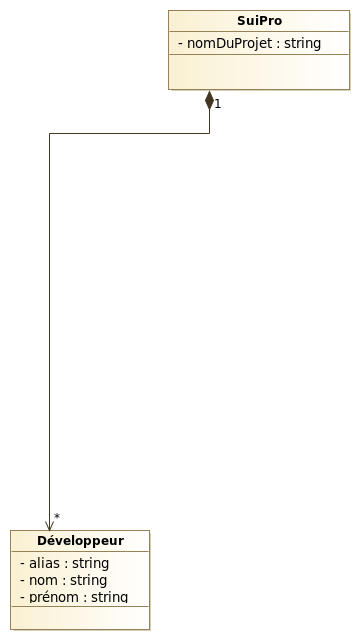
\includegraphics[scale=0.6]{Diagrammes/suipro_uml_diag_classes}
\caption{Diagramme de classes.}
\end{center}
\label{umlet_diag_classes}
\end{figure}

\newpage

\subsection{Diagrammes de séquence}

{\noindent\color{red}\textbf{La section est à compléter avec les
    diagrammes de séquence de vos cas d'utilisation les plus
    importants, c'est-à-dire avec ceux de priorité haute. Ce
    commentaire est à retirer ensuite.}}

\begin{compactitem}
\item arguments en entrée: l'alias du développeur, et le nom et le
  prénom du développeur
\item rappel de la précondition: alias bien formé (non \nullvalue et
  non vide) $\land$ nom bien formé (non \nullvalue et non vide)
  $\land$ prénom bien formé (non \nullvalue et non vide) $\land$
  développeur avec cet identifiant inexistant
\item algorithme:
\begin{compactenum}
\item vérifier les arguments
\item chercher un développeur avec cet alias
\item vérifier que le développeur est inexistant
\item instancier le développeur
\item ajouter le développeur dans la collection des développeurs
\end{compactenum}
\end{compactitem}

\begin{figure}[ht!]
\begin{center}
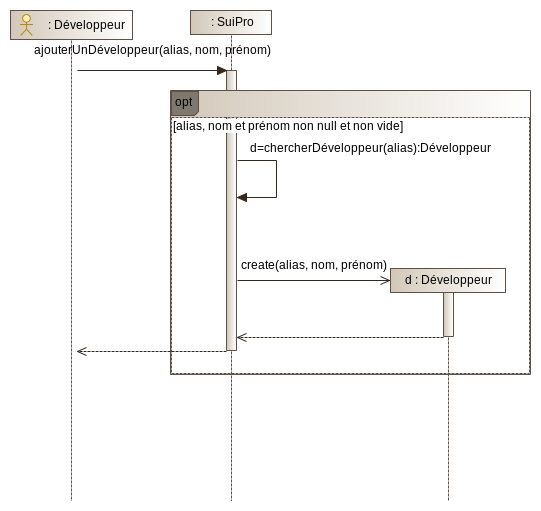
\includegraphics[scale=0.6]{./Diagrammes/suipro_uml_diag_seq_ajouter_developpeur}
\caption{Diagramme de séquence du cas d'utilisation <<~ajouter un
  développeur~>>}
\end{center}
\label{umlet_diag_sequence_ajouter_developpeur}
\end{figure}

\newpage

\section{Diagrammes de machine à états et invariants}

\subsection{Classe \textsf{Développeur}}

{\noindent\color{red}\textbf{La section est à mettre à jour. Ce
    commentaire est à retirer ensuite.}}

\begin{figure}[ht!]
\begin{center}
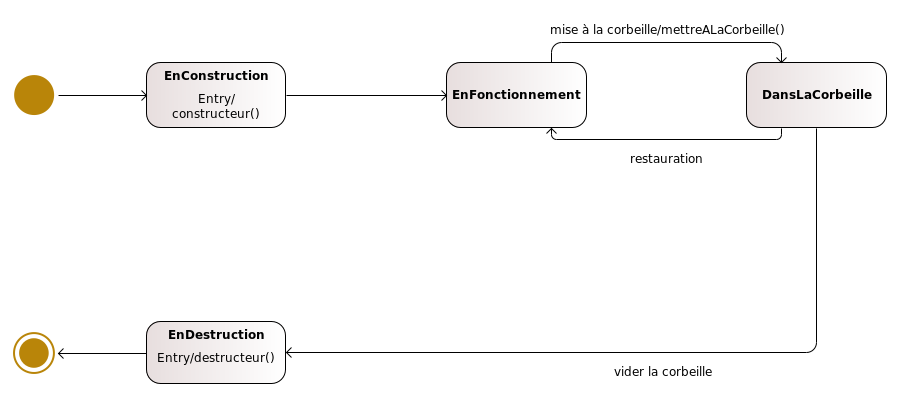
\includegraphics[scale=0.5]{./Diagrammes/suipro_uml_diag_machine_a_etats_developpeur}
\caption{Diagramme de machine à états de la classe \texttt{Développeur}}
\end{center}
\label{umlet_diag_machine_a_etats_developpeur}
\end{figure}

\newcommand{\emptystring}{\ensuremath\mathrm{vide}}
\newcommand{\alias}{\ensuremath\mathrm{alias}}
\newcommand{\nom}{\ensuremath\mathrm{nom}}
\newcommand{\prenom}{\ensuremath\mathrm{prenom}}
L'invariant de la classe \textsf{Développeur} est le suivant:
\begin{tabbing}
M \= M \= M \= M \= M \= M \= M \kill
\> $\land$ \> $\alias \neq \nullvalue \land \alias \neq \emptystring$\\
\> $\land$ \> $\nom \neq \nullvalue \land \nom \neq \emptystring$\\
\> $\land$ \> $\prenom \neq \nullvalue \land \prenom \neq \emptystring$\\
\end{tabbing}

\newpage

\subsection{Classes \textsf{Tâche}}

{\noindent\color{red}\textbf{La section est à compléter. Ce
    commentaire est à retirer ensuite.}}

\begin{figure}[ht!]
\begin{center}
%\includegraphics[scale=0.5]{Diagrammes/suipro_uml_diag_machine_a_etats_tache}
\caption{Diagramme de machine à états de la classe \texttt{Tâche}.}
\end{center}
\label{umlet_diag_machine_a_etats_envoi}
\end{figure}

L'invariant de la classe \textsf{Tâche} est le suivant:
%% \begin{tabbing}
%% M \= M \= M \= M \= M \= M \= M \kill
%% \> $\land$ \>
%% \> $\land$ \>
%% \> $\land$ \>
%% \> $\land$ \>
%% \> $\land$ \>
%% \end{tabbing}

\newpage

\section{Fiche des classes}

\subsection{Classe \textsf{Développeur}}

{\noindent\color{red}\textbf{La section est à mettre à jour. Ce
    commentaire est à retirer ensuite.}}

\begin{center}
\begin{longtable}{|p{12cm}|}
\hline
\multicolumn{1}{|c|}{{\Large \textsf{Développeur}}} \\
\hline
\cmt{attributs <<~association~>>} \\
$-$ periodesDeTravail : Liste<PeriodeDeTravail>\\
\cmt{attributs <<~modifiables~>>}\\
$-$ alias : String \\
$-$ nom : String \\
$-$ prénom : String \\
\hline
\cmt{opérations} \\
$+$ constructeur(String identifiant, String description) \\
$+$ invariant() : boolean \\
$+$ getIdentifiant() : String \\
$+$ getDescription() : String \\
$+$ afficher() : List<String> \\
\hline
\end{longtable}
\end{center}

\newpage

\subsection{Classe \textsf{Tâche}}

{\noindent\color{red}\textbf{La section est à compléter. Ce
    commentaire est à retirer ensuite.}}

\newpage

\section{Préparation des tests unitaires}

\subsection{Classe \textsf{Développeur}}

{\noindent\color{red}\textbf{La section est à mettre à jour. Ce
    commentaire est à retirer ensuite.}}

\begin{table}[!ht]
\begin{center}
\begin{tabular}{|p{0.6\linewidth}|c|c|c|c|}
\hline
Numéro de test
&1&2&3&4\\
\hline
\hline
\texttt{alias} $\neq \nullvalue \land \neg \emptystring$
&F&T&T&T\\
\hline
\texttt{nom} $\neq \nullvalue \land \neg \emptystring$
& &F&T&T\\
\hline
\texttt{prenom} $\neq \nullvalue \land \neg \emptystring$
& & &F&T\\
\hline
\hline
$\alias' = \alias$
& & & &T\\
\hline
$\nom' = \nom$
& & & &T\\
\hline
$\prenom' = \prenom$
& & & &T\\
\hline
$\invariant$
& & & &T\\
\hline
Levée d'une exception&\textsc{oui}&\textsc{oui}&\textsc{oui}&\textsc{non}\\
\hline
\hline
Objet créé
&F&F&F&T\\
\hline
\hline
Nombre de jeux de test 
&2&2&2&1\\
\hline
\end{tabular}
\caption{Méthode \texttt{constructeur} de la classe
  \texttt{Développeur}}
\end{center}
\end{table}

\subsection{Classe \textsf{Tâche}}

{\noindent\color{red}\textbf{La section est à compléter. Ce
    commentaire est à retirer ensuite.}}

\end{document}
